\chapter{Arquitetura}

% \begin{figure}[!h]
%  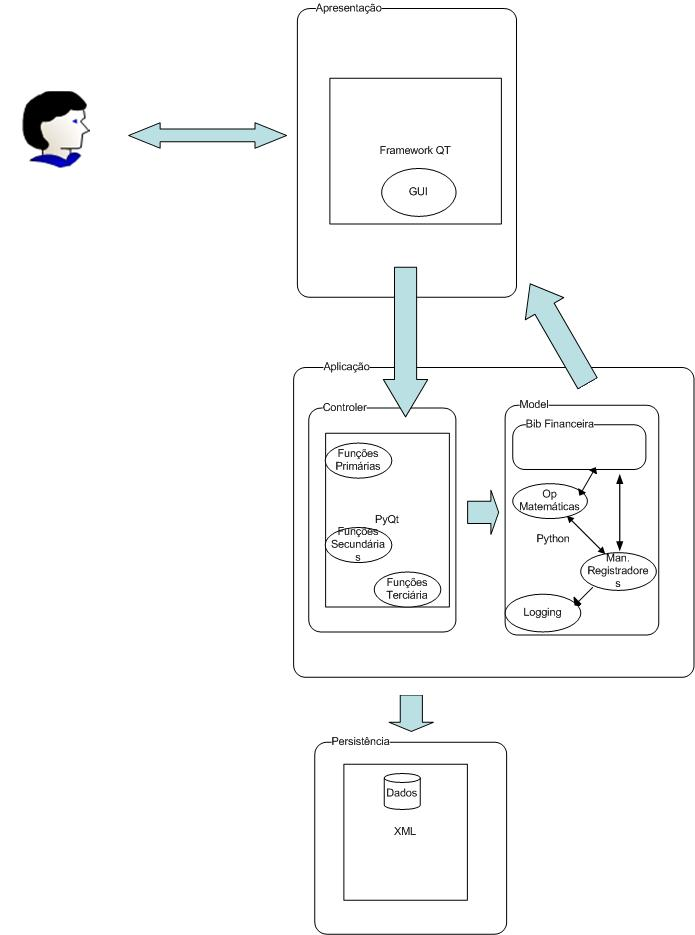
\includegraphics[scale=0.5]{arquitetura.jpg}
%  \caption{\it Projeto arquitetural da aplicação.} \label{fig:arquit}
% \end{figure}

\section{Descrição da Arquitetura}

O sistema proposto foi idealizado para funcionar localmente no dispositivo N800 da Nokia, funcionando no modo monousuário. O sistema pode ser dividido, em três camadas lógicas que serão conectadas através do padrão MVC \cite{mvc}, conforme pode ser visto na Figura \ref{fig:arquit}:
\begin{itemize}
 \item \textbf{Apresentação}: camada que é responsável por lidar com todo aspecto de interface para interação com o usuário.
 \item \textbf{Aplicação}: camada que é responsável por conter toda a lógica do negócio da aplicação, mantendo, assim total desacoplamento com as demais camadas.
 \item \textbf{Persistência}: camada que é responsável por lidar com toda a persistência de dados de modo que eles possam ser usados posteriormente de forma íntegra.
\end{itemize}

Vale lembrar que toda a comunicação entre essas camadas, bem como entre os diversos módulos internos as mesmas, é realizada através de um conjunto de interfaces bem definidas, buscando assim, garantir flexibilidade e baixo acoplamento, bem como um eventual reuso e/ou substituição da biblioteca financeira em questão. A separação entre os módulos se deu da forma mais simplificada possível para que, independente da sobrecarga existente, esta não influenciasse fortemente o tempo de resposta desejado para as interações com o usuário da aplicação, este foi um dos requisitos não funcionais especificados na fase de análise.
Outro ponto importante a se destacar é o uso do paradigma OO, bem como do uso de scripts, dada a escolha da linguagem Python para o desenvolvimento da Camada de Aplicação.

\begin{figure}[!h]
 \centering
 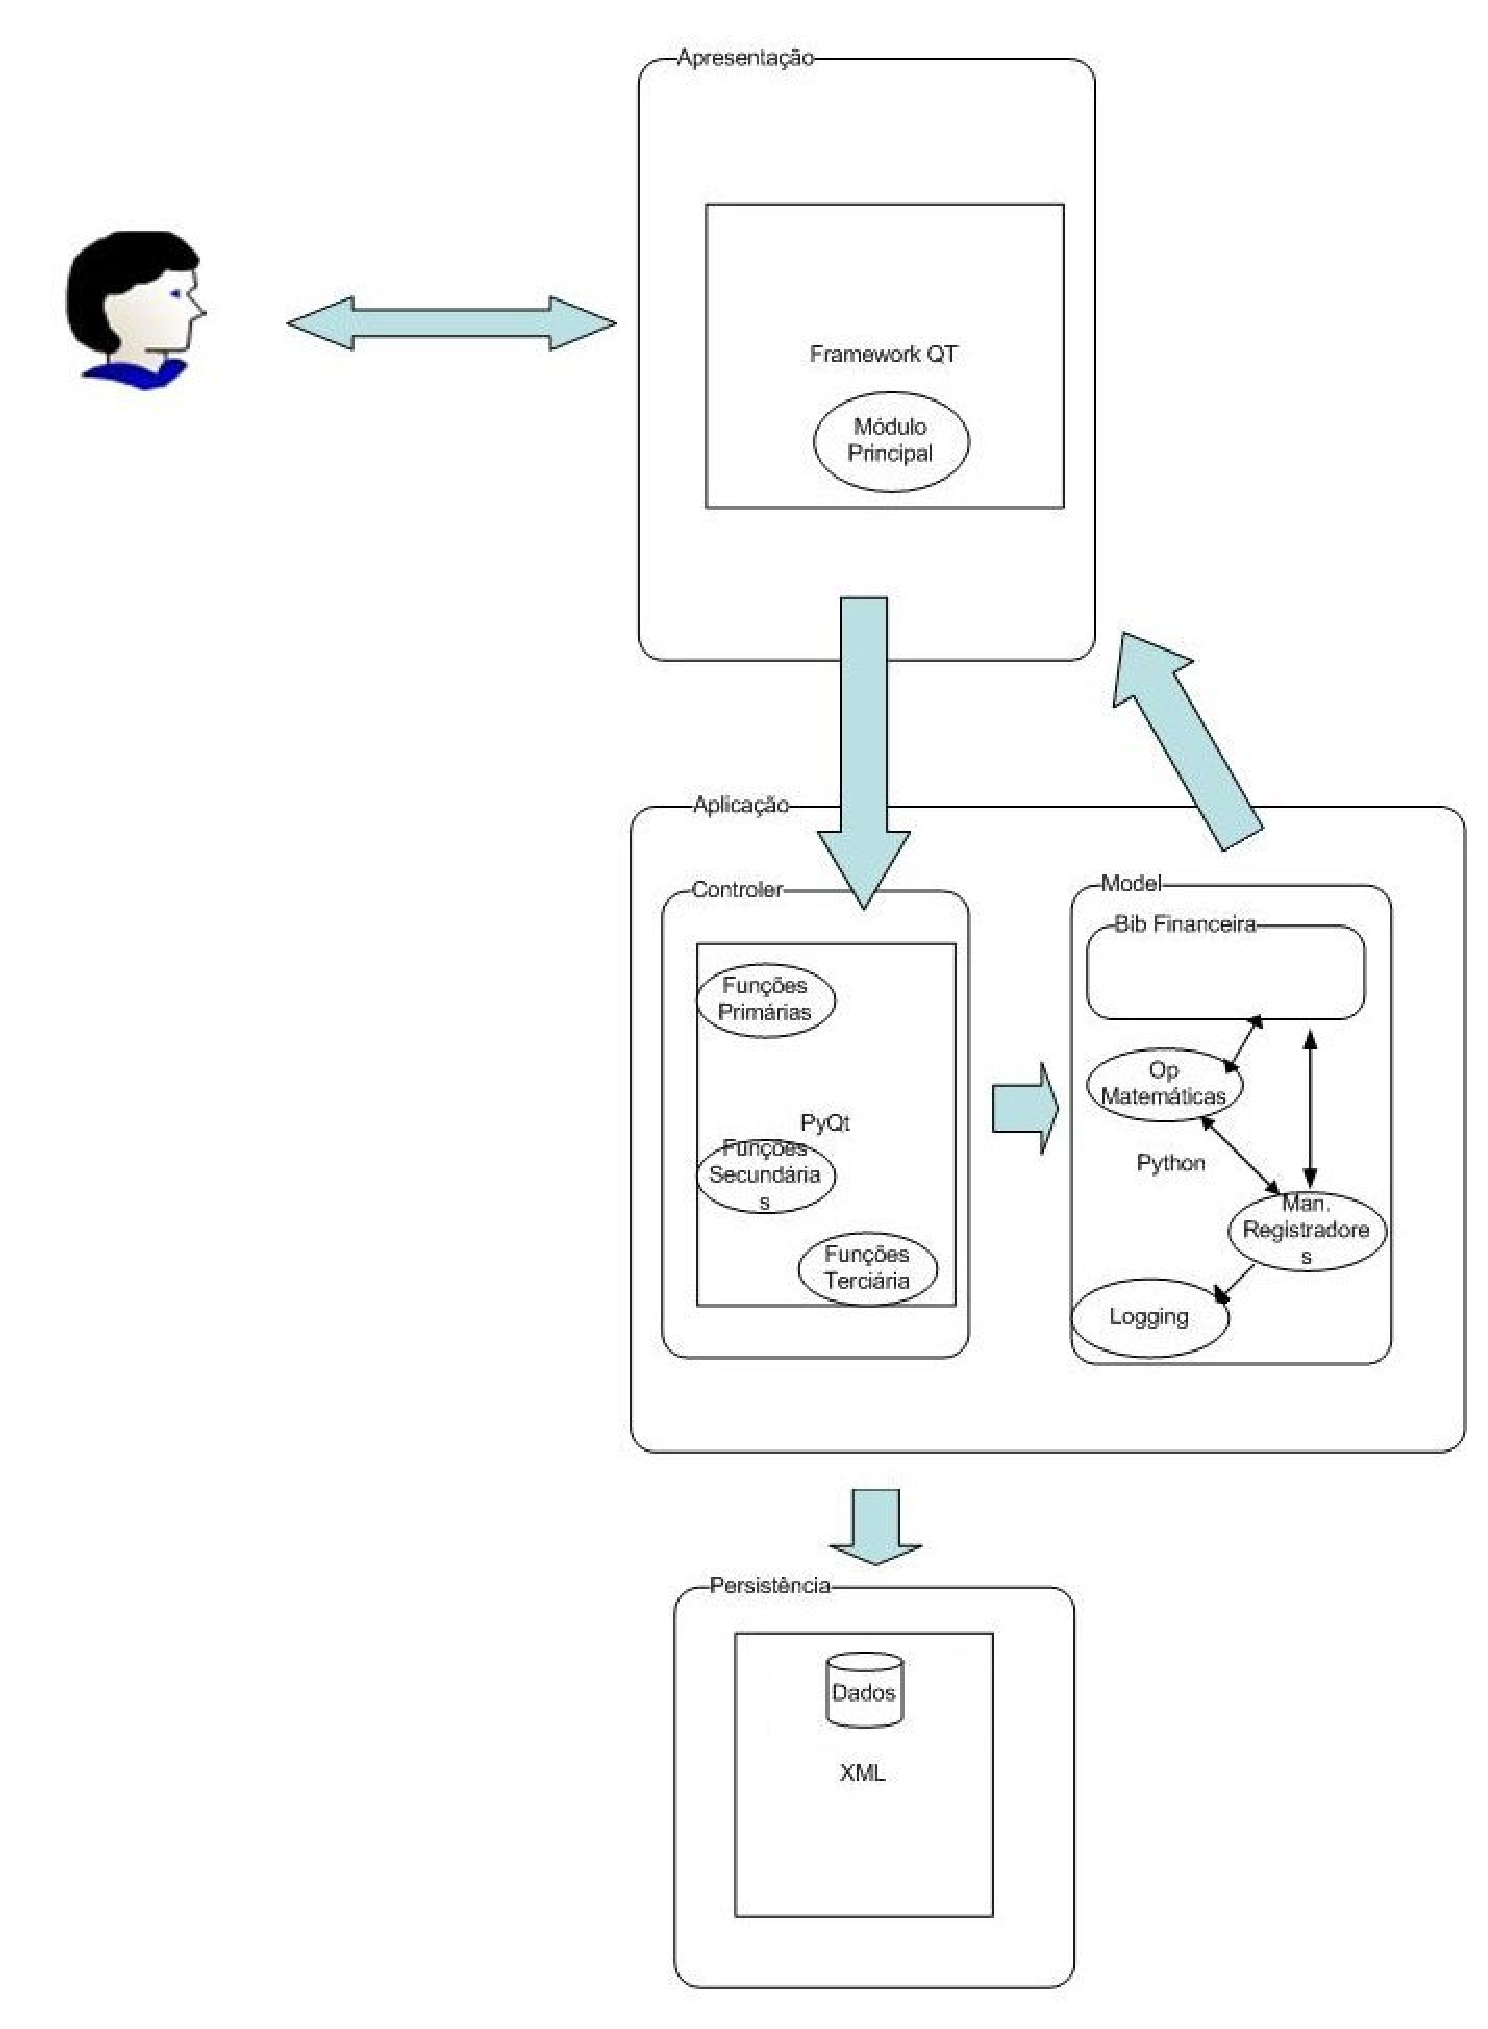
\includegraphics[scale=0.5]{arquitetura.eps}
 \caption{\it Projeto arquitetural da aplicação.} \label{fig:arquit}
\end{figure}

\subsection{Camada de Apresentação}
O sistema é acessado localmente por um único usuário, via uma interface similar à da calculadora financeira que está sendo usada como base, tendo a opção de finalização da aplicação através de um botão. É importante destacar ainda que toda entrada realizada pelo usuário se dá através da interface \textit{touch-screen} disponibilizada pelo dispositivo selecionado.
Para o desenvolvimento dessa camada fez-se uso do \textit{Framework QT}, com auxílio da ferramenta de design gráfico \textit{QT Designer}. É de suma importância aqui o desenvolvimento de \textit{packages} no que diz respeito aos componentes visuais da calculadora, por exemplo, os botões da mesma.

\subsection{Camada de Aplicação}
Como dito anteriormente, essa camada é responsável por toda a lógica de negócio do sistema e foi desenvolvida em Python devido a suas vantagens na manipulação de números.
Dentre os principais componentes desta camada pode-se dar destaque à biblioteca financeira (também desenvolvida pela equipe com o foco de ser um módulo importável que contenha essencialmente funcionalidades financeiras), ao módulo de operações matemáticas, ao módulo de gerenciamento dos registradores existentes (responsável por fornecer os dados a serem persistidos) e ao módulo de comunicação com a interface da calculadora.
 Dentro dessa camada pode-se destacar que as interações ocorrem em duas etapas:
\begin{enumerate}
 \item Numa primeira etapa tem-se a comunicação dessa camada com a camada de apresentação do sistema através dos controladores, fazendo estes uso dos \textit{bindings} em PyQt e sendo subdivididos de acordo com as funcionalidades providas por cada tecla.
 \item Numa segunda etapa observa-se:	
 \begin{itemize}
    \item A comunicação dos módulos controladores com o restante da lógica da aplicação, fazendo uso das funcionalidades da biblioteca financeira, do módulo matemático e manipulando os seus registradores.
    \item A interação entre os registradores e a biblioteca, onde os primeiros podem fornecer entradas para a última, a interação entre os registradores e o módulo matemático e a interação entre o módulo matemático e a biblioteca.
 \end{itemize}
\end{enumerate}

\subsection{Camada de Persistência}
A persistência dos dados relativos aos registradores é realizada através do uso de arquivos. Os dados que são armazenados nos arquivos são recarregados sempre que houver a inicialização da aplicação, demandando, assim, pouca interação com o disco.
Outro aspecto relevante a ser considerado aqui é a segurança do sistema.  Devido à natureza do sistema focou-se nos aspectos de integridade dos dados manipulados, fazendo com que os arquivos utilizados fossem armazenados de forma oculta ao usuário, evitando, assim, alterações dos mesmos por parte deste.

\subsection{\textit{Packaging}}
Foi tomada a decisão de distribuir a aplicação através de um arquivo de instalação de extensão \textit{.deb}, simplificando, assim, a maneira de instalação do software. Tal arquivo, futuramente, poderá ser obtido por download de certo servidor web que será escolhido pela equipe em conjunto com o cliente.

\subsection{Pontos Adicionais}
Com relação à integração com outras aplicações, é do interesse da equipe que a biblioteca financeira desenvolvida possa vir a ser usada por outros desenvolvedores como um dos vários módulos que auxiliem sua aplicação específica.
Por fim, todo o desenvolvimento foi guiado pelo padrão de operações que é usado pela HP12-C que é a Notação Polonesa Reversa (ou Notação Polonesa Inversa segundo alguns autores \cite{NPR}).